\documentclass[crop,tikz]{standalone}

\usepackage{graphicx}
\usepackage{fancybox}
\usepackage{amsmath, amssymb}

\newcommand{\calP}{\mathcal{P}}
\newcommand{\bbR}{\mathbb{R}}
\DeclareMathOperator*{\argmax}{argmax}
\DeclareMathOperator*{\argmin}{argmin}

\usetikzlibrary{positioning}

\begin{document}

\begin{tikzpicture}
    \node (start) at (0, 0) {};
    \node[right = 80pt of start] (encoder) {\ovalbox{\begin{Bcenter} GLM \\ $\varphi_w$ \end{Bcenter}}};
    \node[right = 80pt of encoder] (optimizer) {\doublebox{\begin{Bcenter} VSP flow \\ Linear Program \end{Bcenter}}};
    \node[right = 80pt of optimizer] (end) {\ovalbox{\begin{Bcenter} Loss \\ function \end{Bcenter}}};

    \draw[->] (start) -- (encoder) node[midway,above] (map_text) {StoVSP} node[midway,below] (map_text2) {instance};
    \draw[->] (encoder) -- (optimizer) node[midway,above] (weights_text) {Edge weights} node[midway,below] (weights_text2) {$\theta_a,\, \forall a\in A$};
    \draw[->] (optimizer) -- (end) node[midway,above] (path_text) {Vehicle routes};

    \node[above = 10pt of map_text, inner sep=0pt] (map) {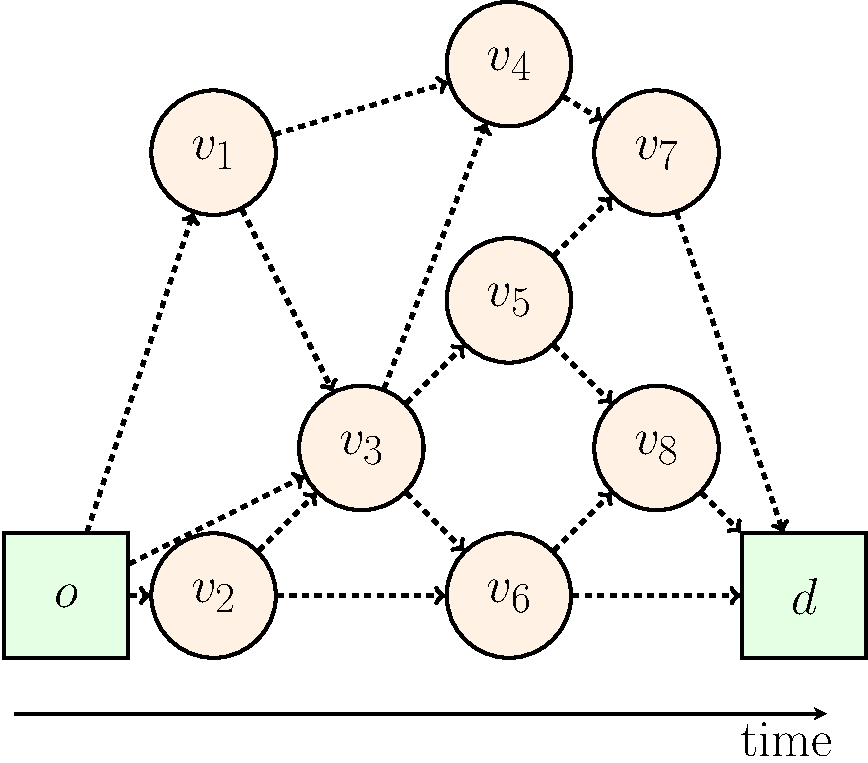
\includegraphics[height=100pt]{./vsp/vsp_instance.pdf}};
    \node[above right = 8.2pt and -18ex of weights_text, inner sep=0pt] (weights) {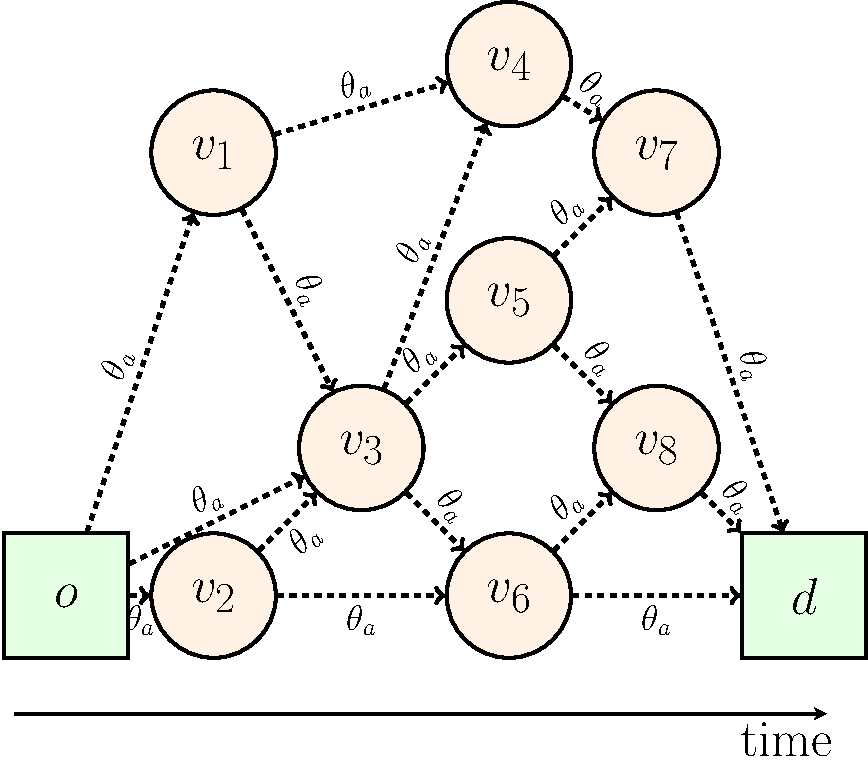
\includegraphics[height=100pt]{./vsp/vsp_weights.pdf}};
    \node[above = 10pt of path_text, inner sep=0pt] (path) {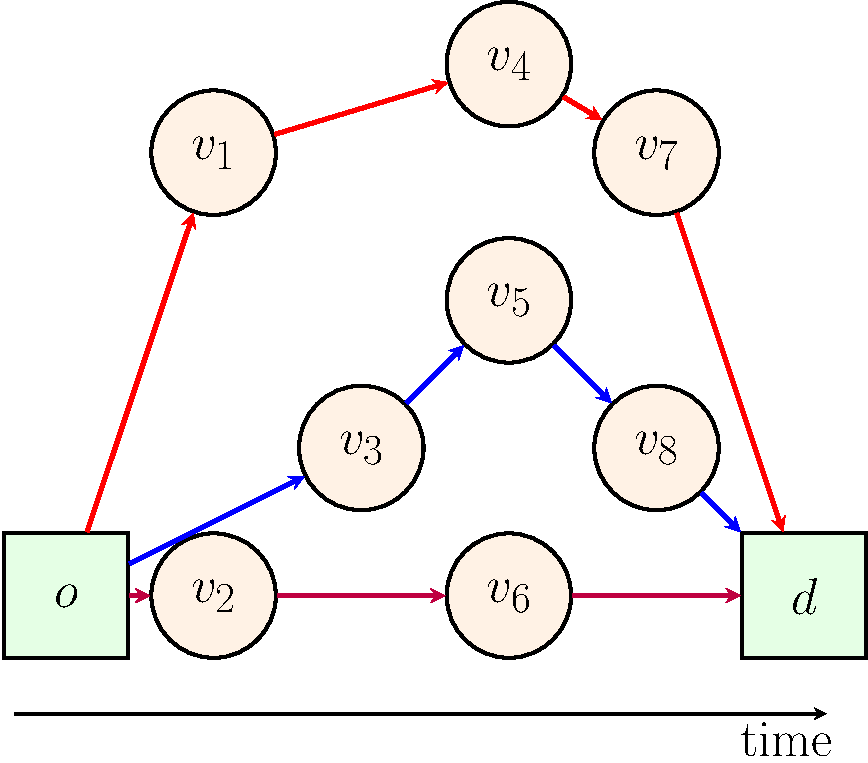
\includegraphics[height=100pt]{./vsp/vsp_solution.pdf}};
\end{tikzpicture}

\end{document}
